\documentclass[12pt, a4paper]{article}
\usepackage[utf8]{inputenc}
% \usepackage[russian]{babel}
\usepackage[pdftex]{graphicx, color}
\usepackage{amsmath, amsfonts, amssymb, amsthm}
\usepackage{bm}
\usepackage[left=2cm,right=2cm,top=1.5cm,bottom=2cm]{geometry}
\usepackage{indentfirst}
\usepackage{hyperref}
\usepackage{textcomp}
\usepackage{float}

\usepackage[table,xcdraw]{xcolor}
\usepackage{diagbox}
\usepackage{tikz}
\usepackage[justification=centering,labelfont=bf]{caption}
\usetikzlibrary{tikzmark}

\graphicspath{{pics/}}

\begin{document}
    \begin{center}
        
\includegraphics[height=3cm]{UVM}

        {\large\textbf{
            CS352 Evolutionary Computation: Homework 1 part 2
        }}

        \vspace{0.3cm}

        \textit{\textbf{Ayat Ospanov}}

        \today
    \end{center}

    \tableofcontents
    \section{Setting the Population Size}\label{sec:pop_setup}
        Let's consider 16-queens problem. In this section we will search for
        a population size that enables us to reliably solve the problem for
        20 repeats for each population size. As the mutation function we
        choose 'swap' mutation.

        Now consider the range of [10, 1400] of population sizes. It was
        chosen as we don't know an appropriate range. To make the program work
        faster, the step of population sizes is 100.

        \begin{figure}[H]
            \centering
            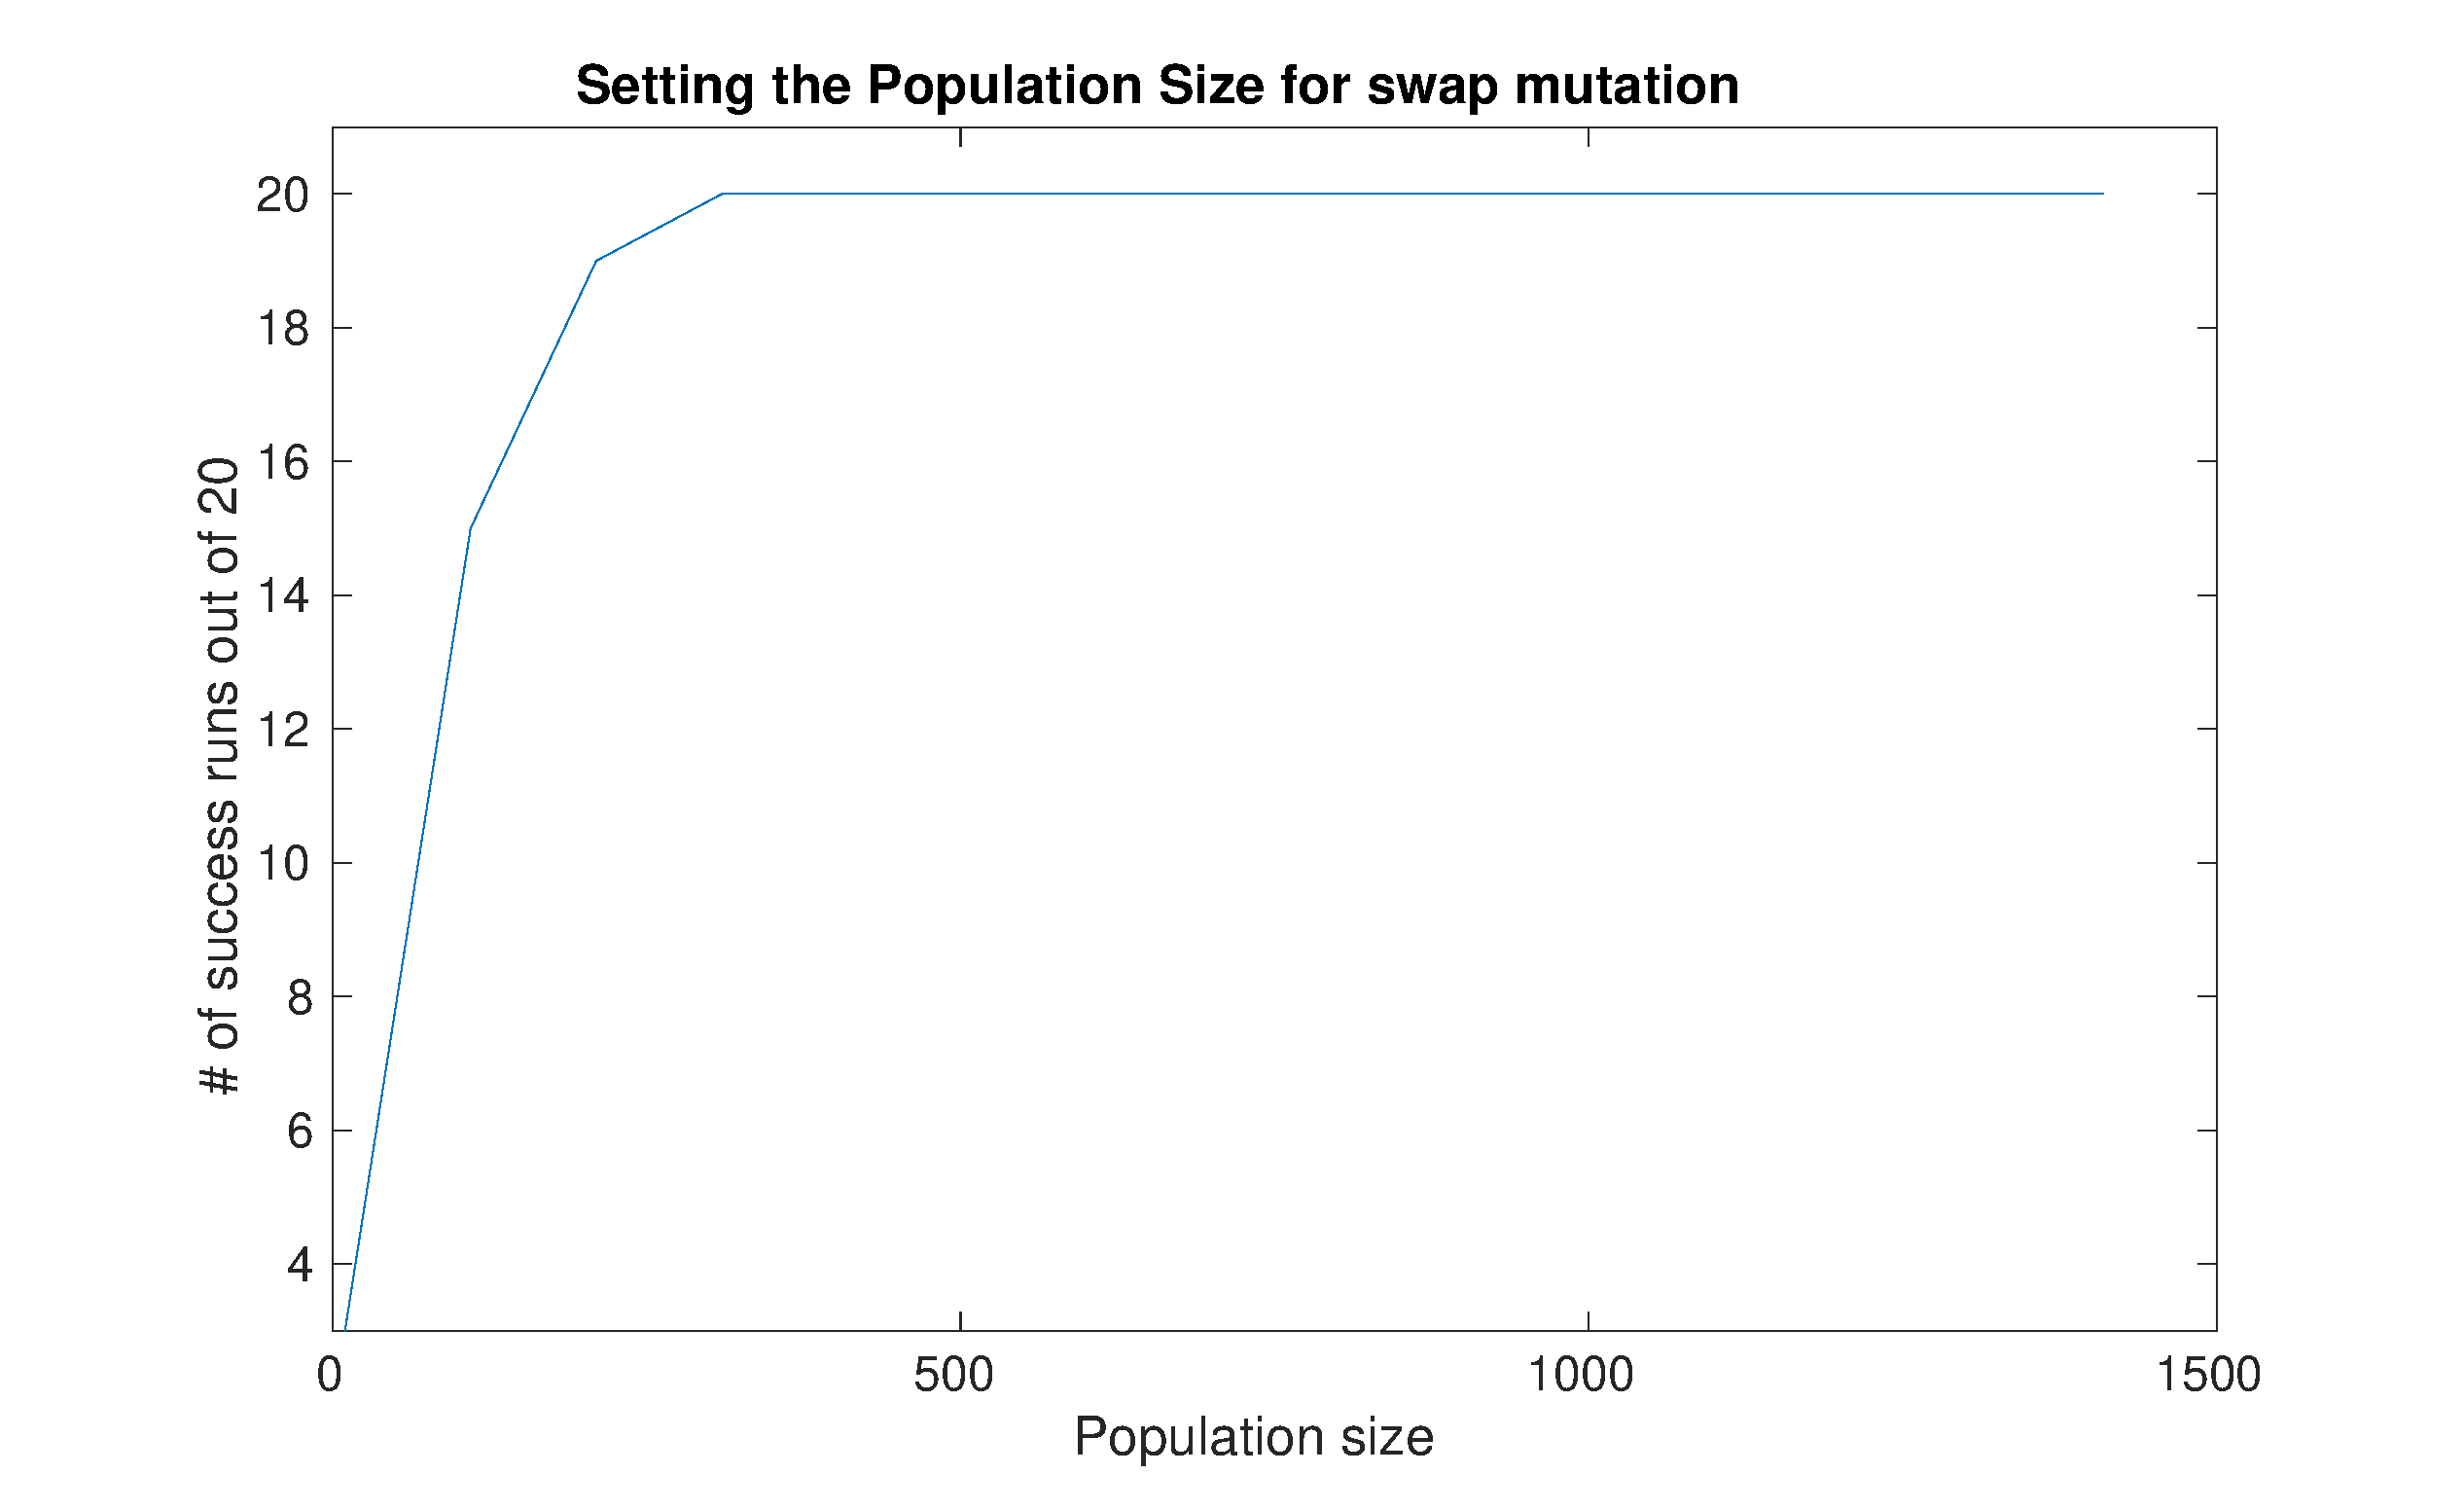
\includegraphics[width=\linewidth]{pop_selection_big.eps}
            \caption{Setting the population size for swap mutation in the range
                of [10, 1400] of population sizes}
            \label{fig:pop_sel_big}
        \end{figure}

        Fig. \ref{fig:pop_sel_big} depicts the number of successful runs out of 20.
        As the plot shows, success rate reaches its maximum of 20/20 between 100
        and 400. Further it stays stable and never drops.

        Therefore, let's narrow in the range of [100, 400] with the step of 10.

        \begin{figure}[H]
            \centering
            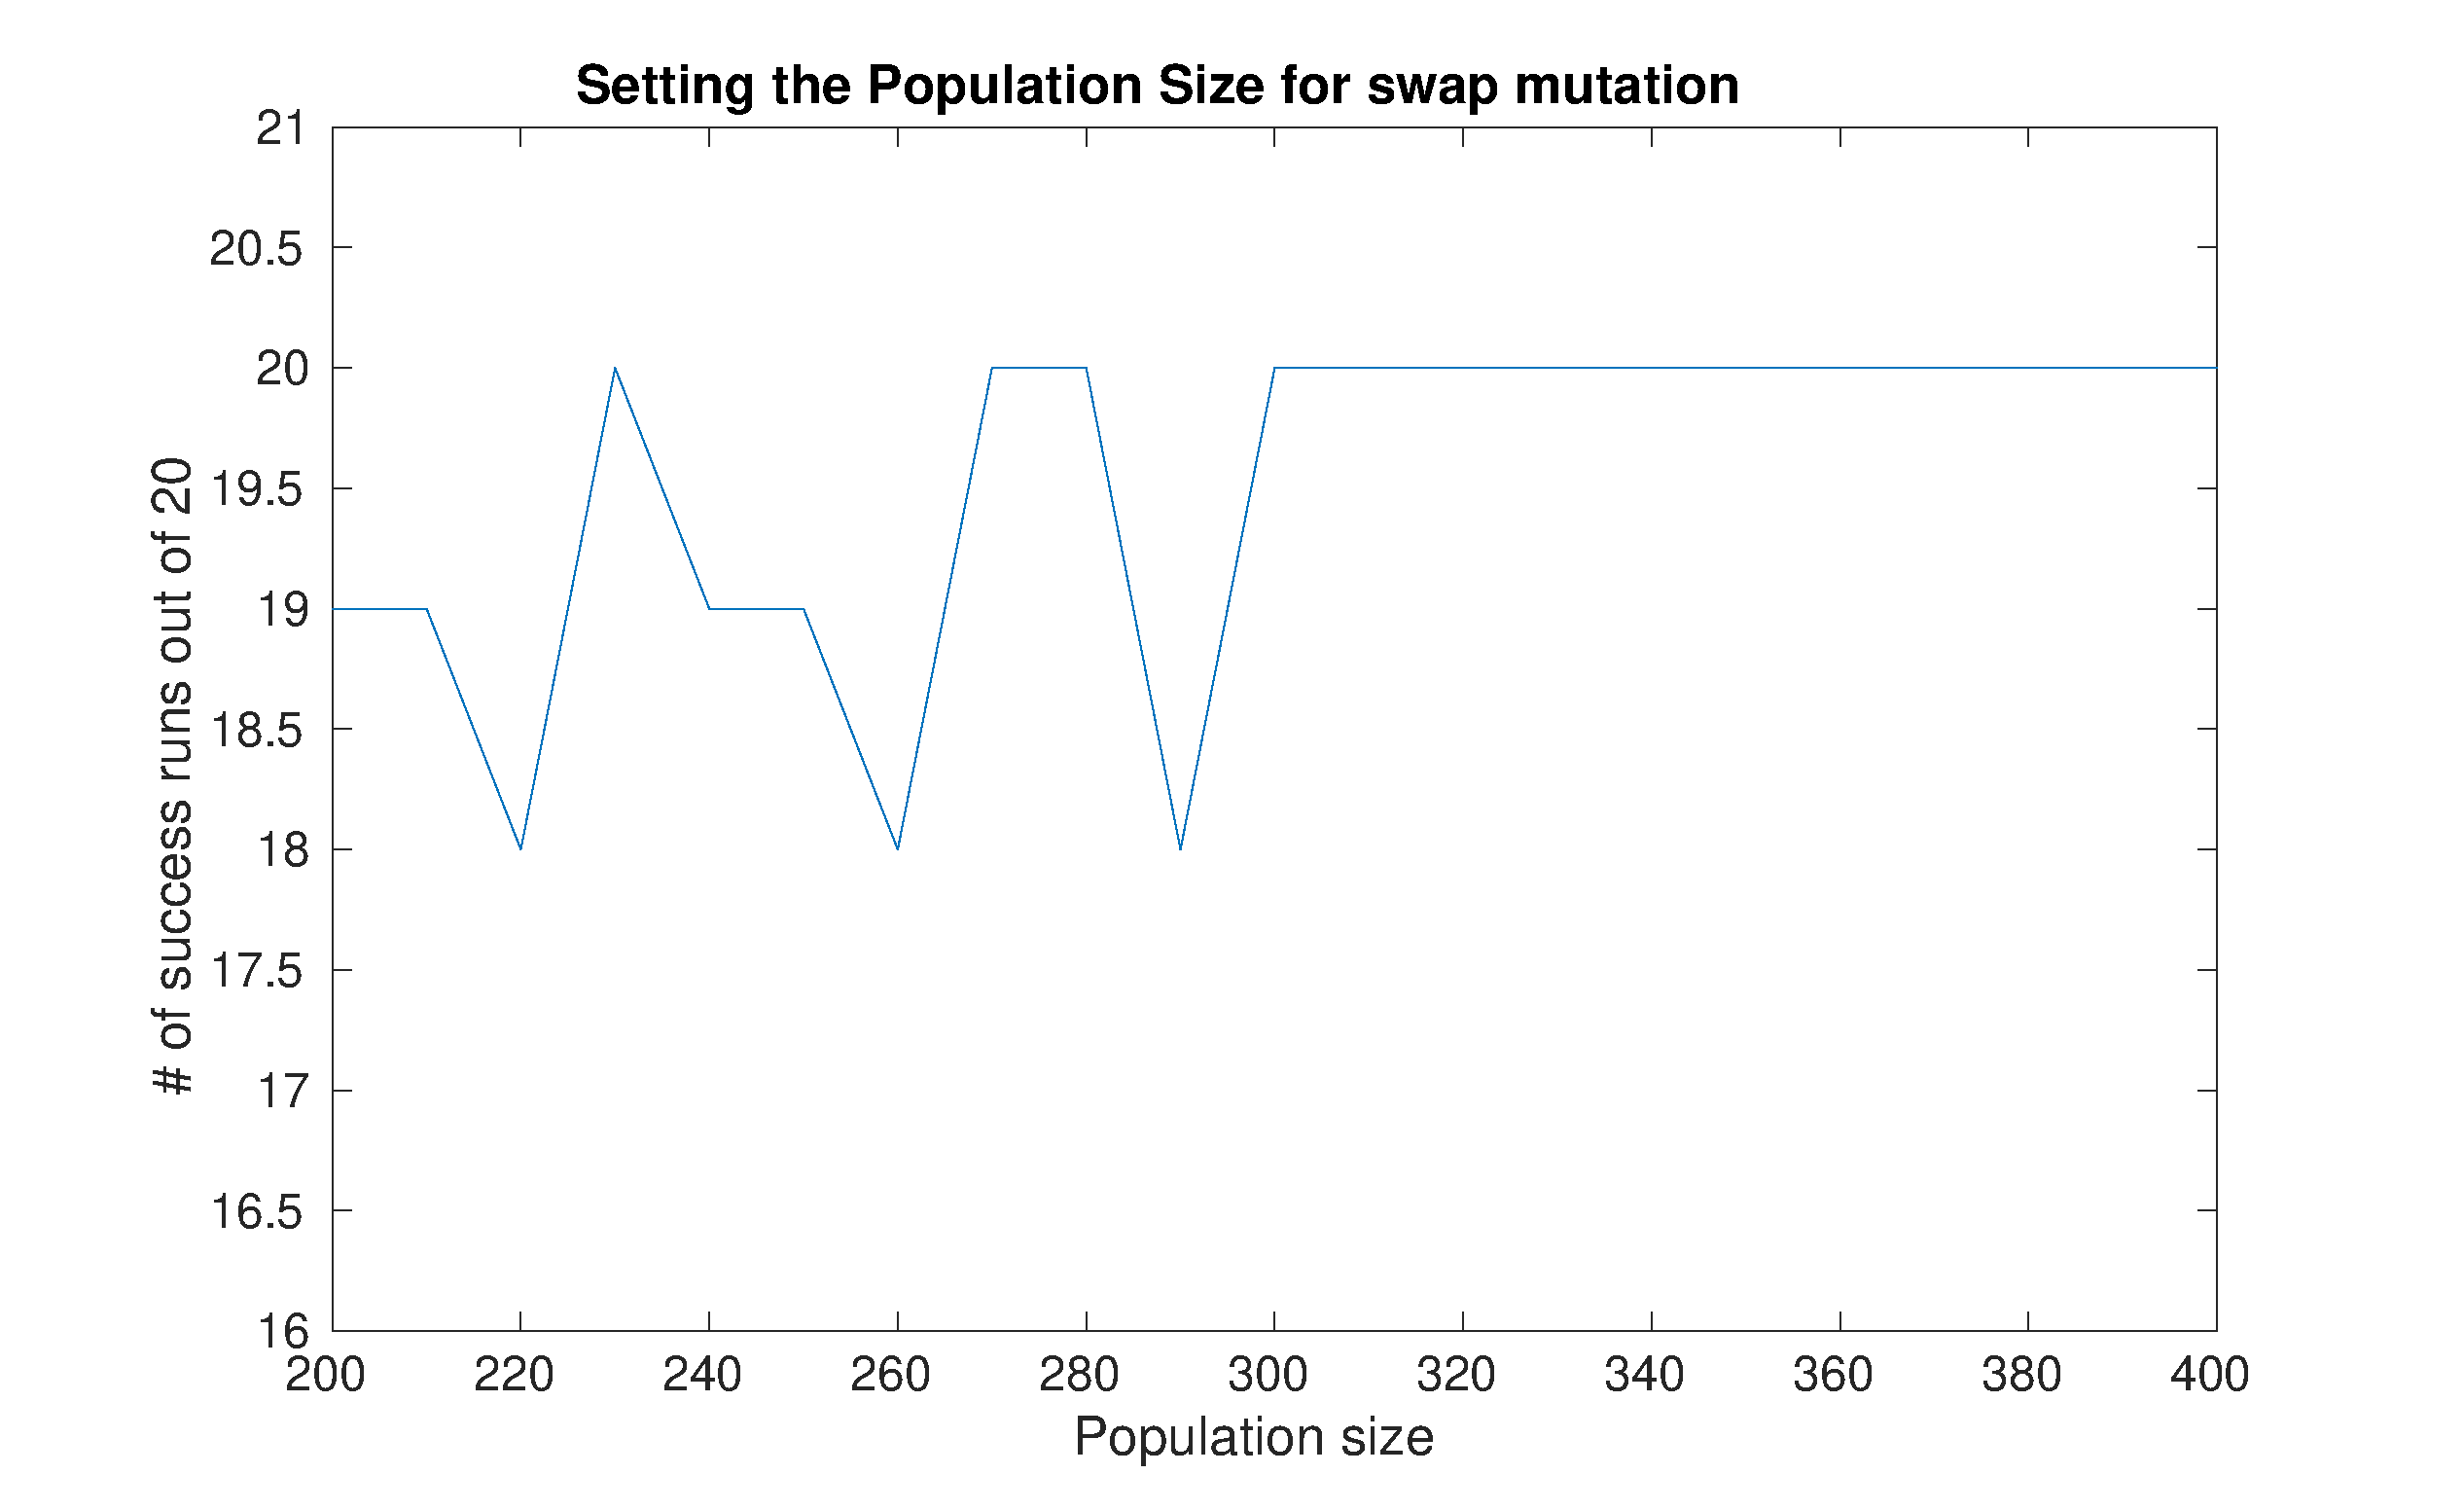
\includegraphics[width=\linewidth]{pop_selection_zoom.eps}
            \caption{Setting the population size for swap mutation in the range
                of [100, 400] of population sizes}
            \label{fig:pop_sel_lil}
        \end{figure}

        As the Fig. \ref{fig:pop_sel_lil} shows, there is a fluctuation of
        success rate between 200 and 300. It was not seen in the wider range
        because we had larger step there. But when we narrowed in, we can see
        the picture in more details. From the plot, it is obvious that starting
        the population size of 300, the line reaches its maximum and becomes
        constant for bigger population sizes.

        Given this information, we can draw a conclusion that the population
        size that enables us to reliably solve the 16-queens problem is 300
        using swap mutation. But as it is the boundary case, it is safer to
        take the population size of 400.

    \section{Mutation functions comparison}
        To compare mutation functions we will use two metrics:
        \begin{itemize}
            \item Success rate over population sizes
            \item Average fitness over generation
        \end{itemize}

        The first metric shows the optimal population size to reliably solve the
        N-queens problem. The less it is the better the function is.

        The second metric shows how fast the algorithm converges while using
        any of mutation functions. It's counted as the average of the best fitnesses
        for 20 runs at each population step.

        Fig. \ref{fig:comp_succ_rate} plots success rate for 20 runs for each
        mutation function. As we found out in the Sec. \ref{sec:pop_setup},
        the appropriate population size for swap mutation is 300. Further success
        rate is constant and on its maximum value.

        Concerning Scramble mutation, its plot fluctuates until the population
        size of 1400. Thus, we can conclude that scramble mutation needs 4 times
        more generation to solve the problem.

        \begin{figure}[H]
            \centering
            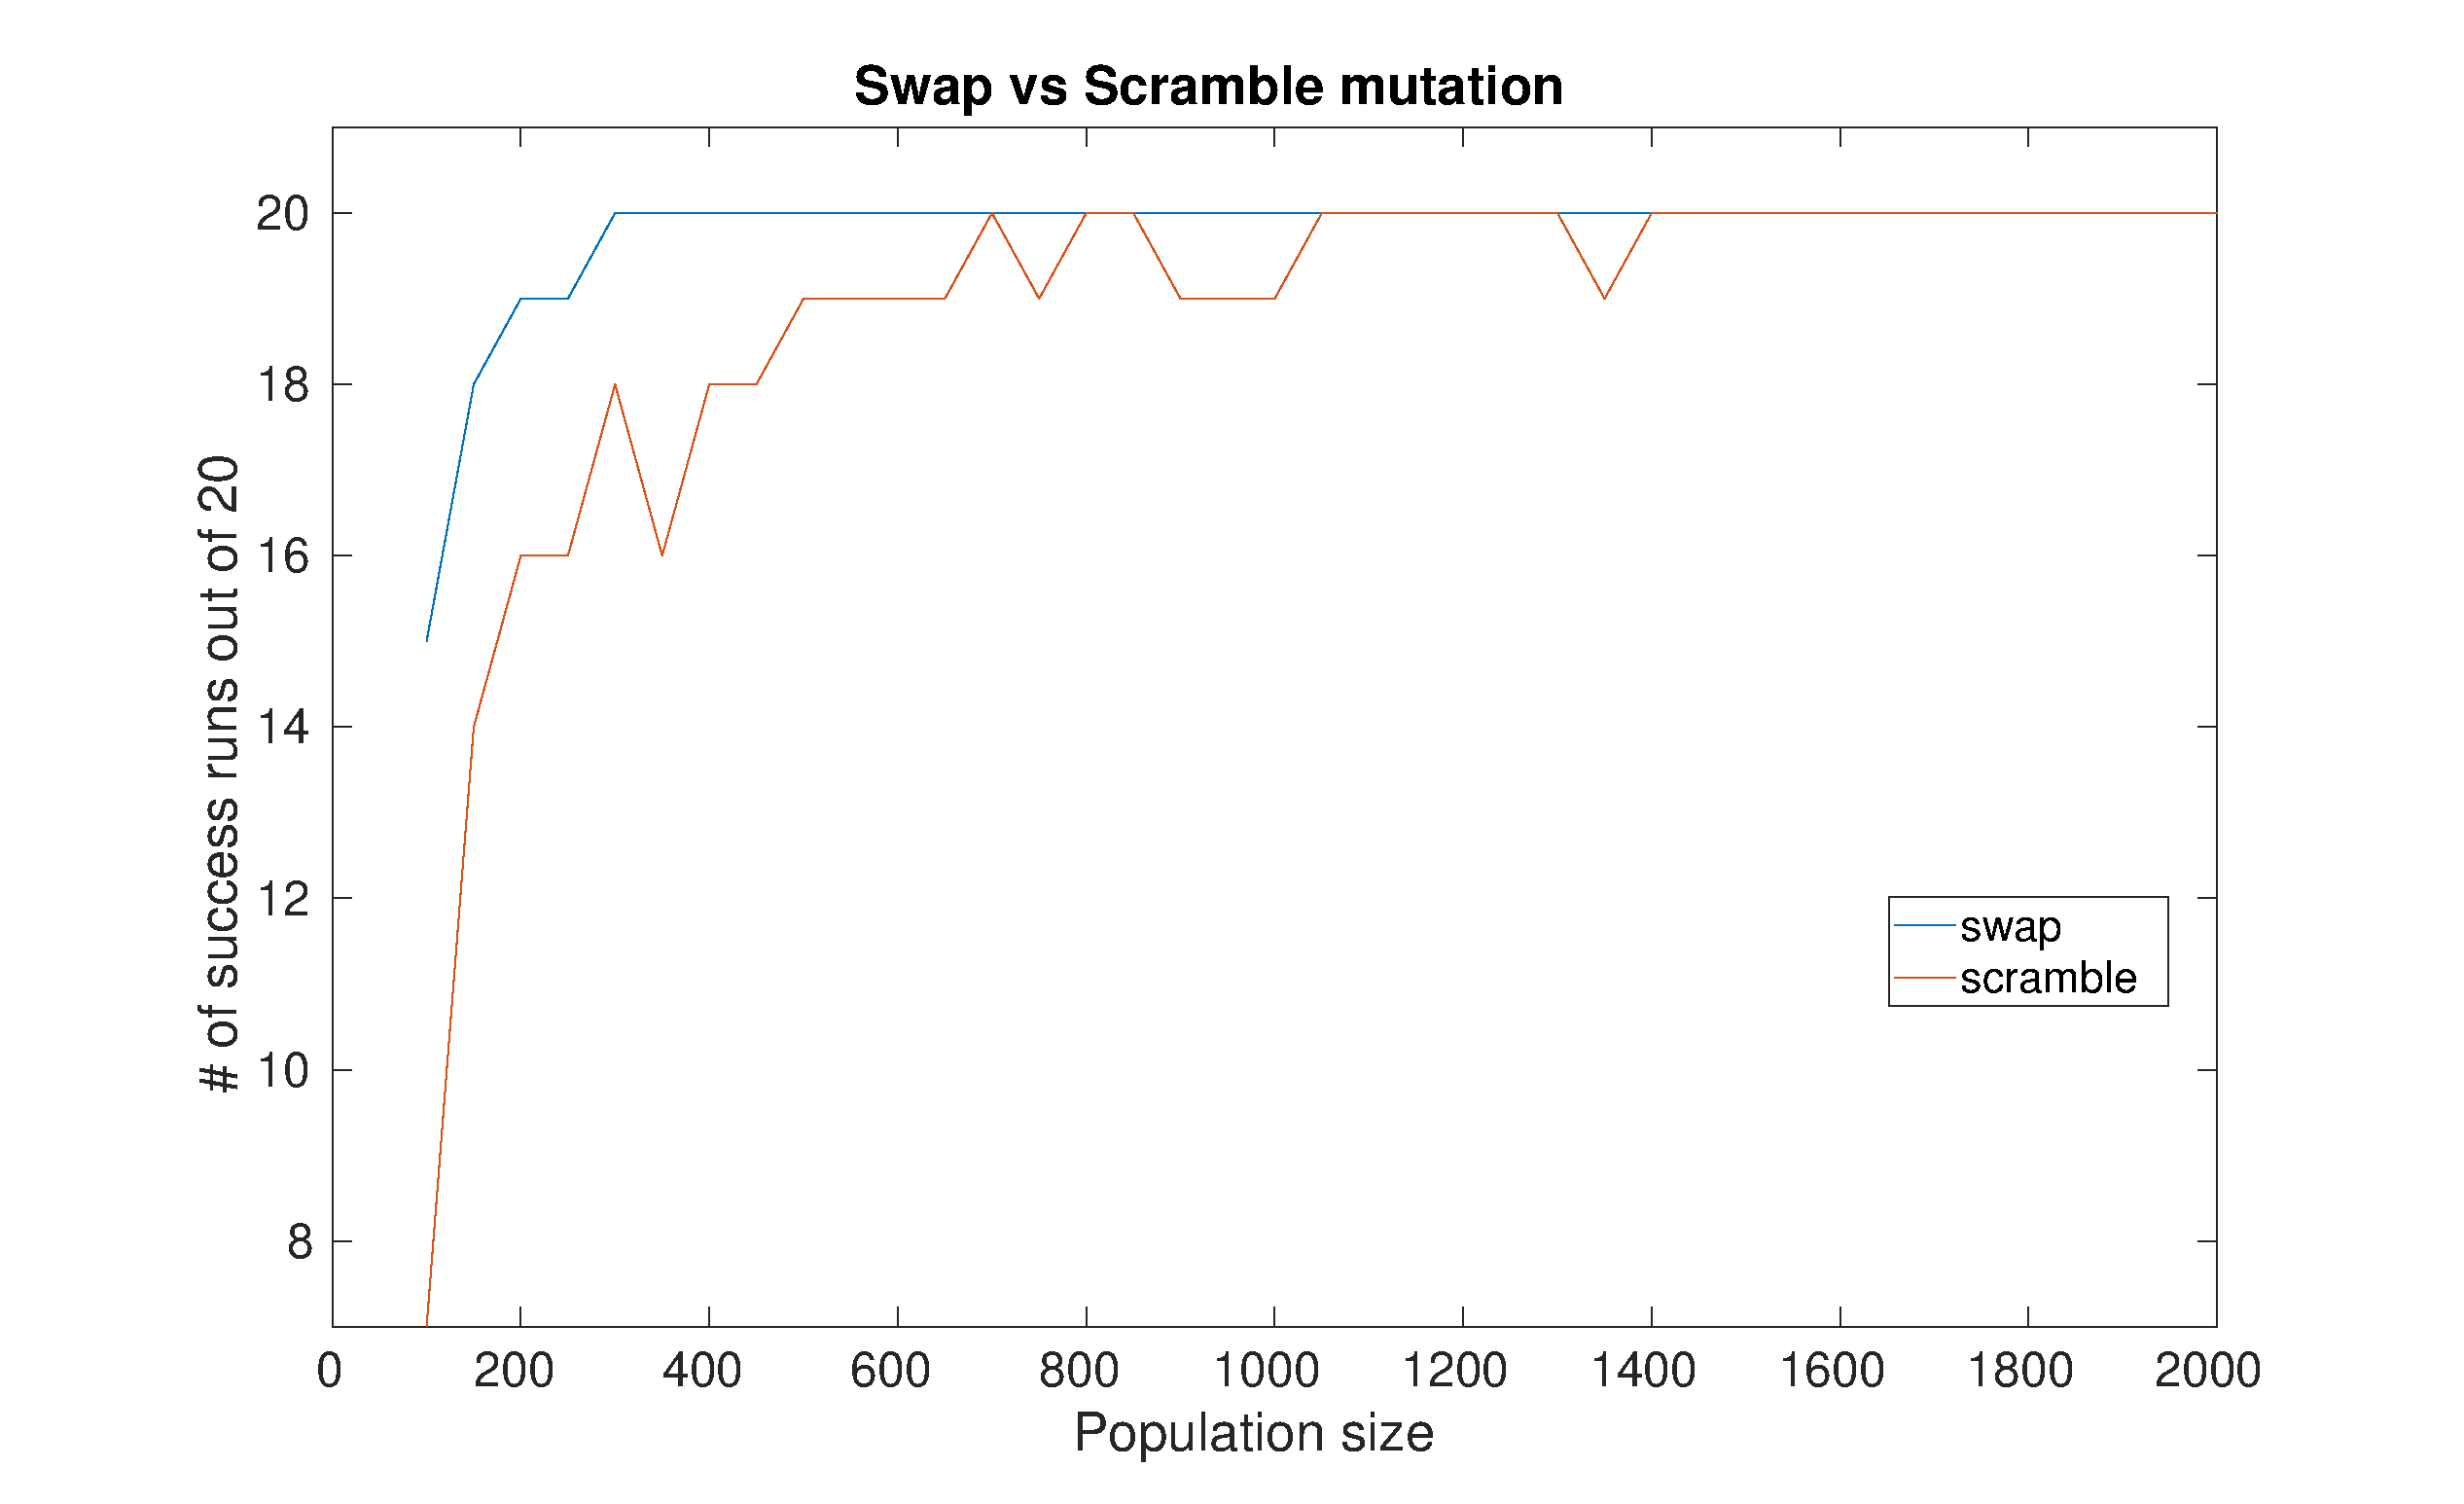
\includegraphics[width=\linewidth]{comparison_success_rate}
            \caption{Mutation functions' comparison by success rate. The range
                of population sizes is [100, 2000]}
            \label{fig:comp_succ_rate}
        \end{figure}

        Fig. \ref{fig:comp_avg_fit} shows average best fitness for 20 runs for
        both of mutation functions. Population size in this case was fixed to
        1400 because for this value both functions work reliably good.

        As it is given in the graph, swap mutation converges in 25 generations,
        while scramble mutation converges in 73 generations. It is about 50
        generations late and 3 times slower.

        \begin{figure}[H]
            \centering
            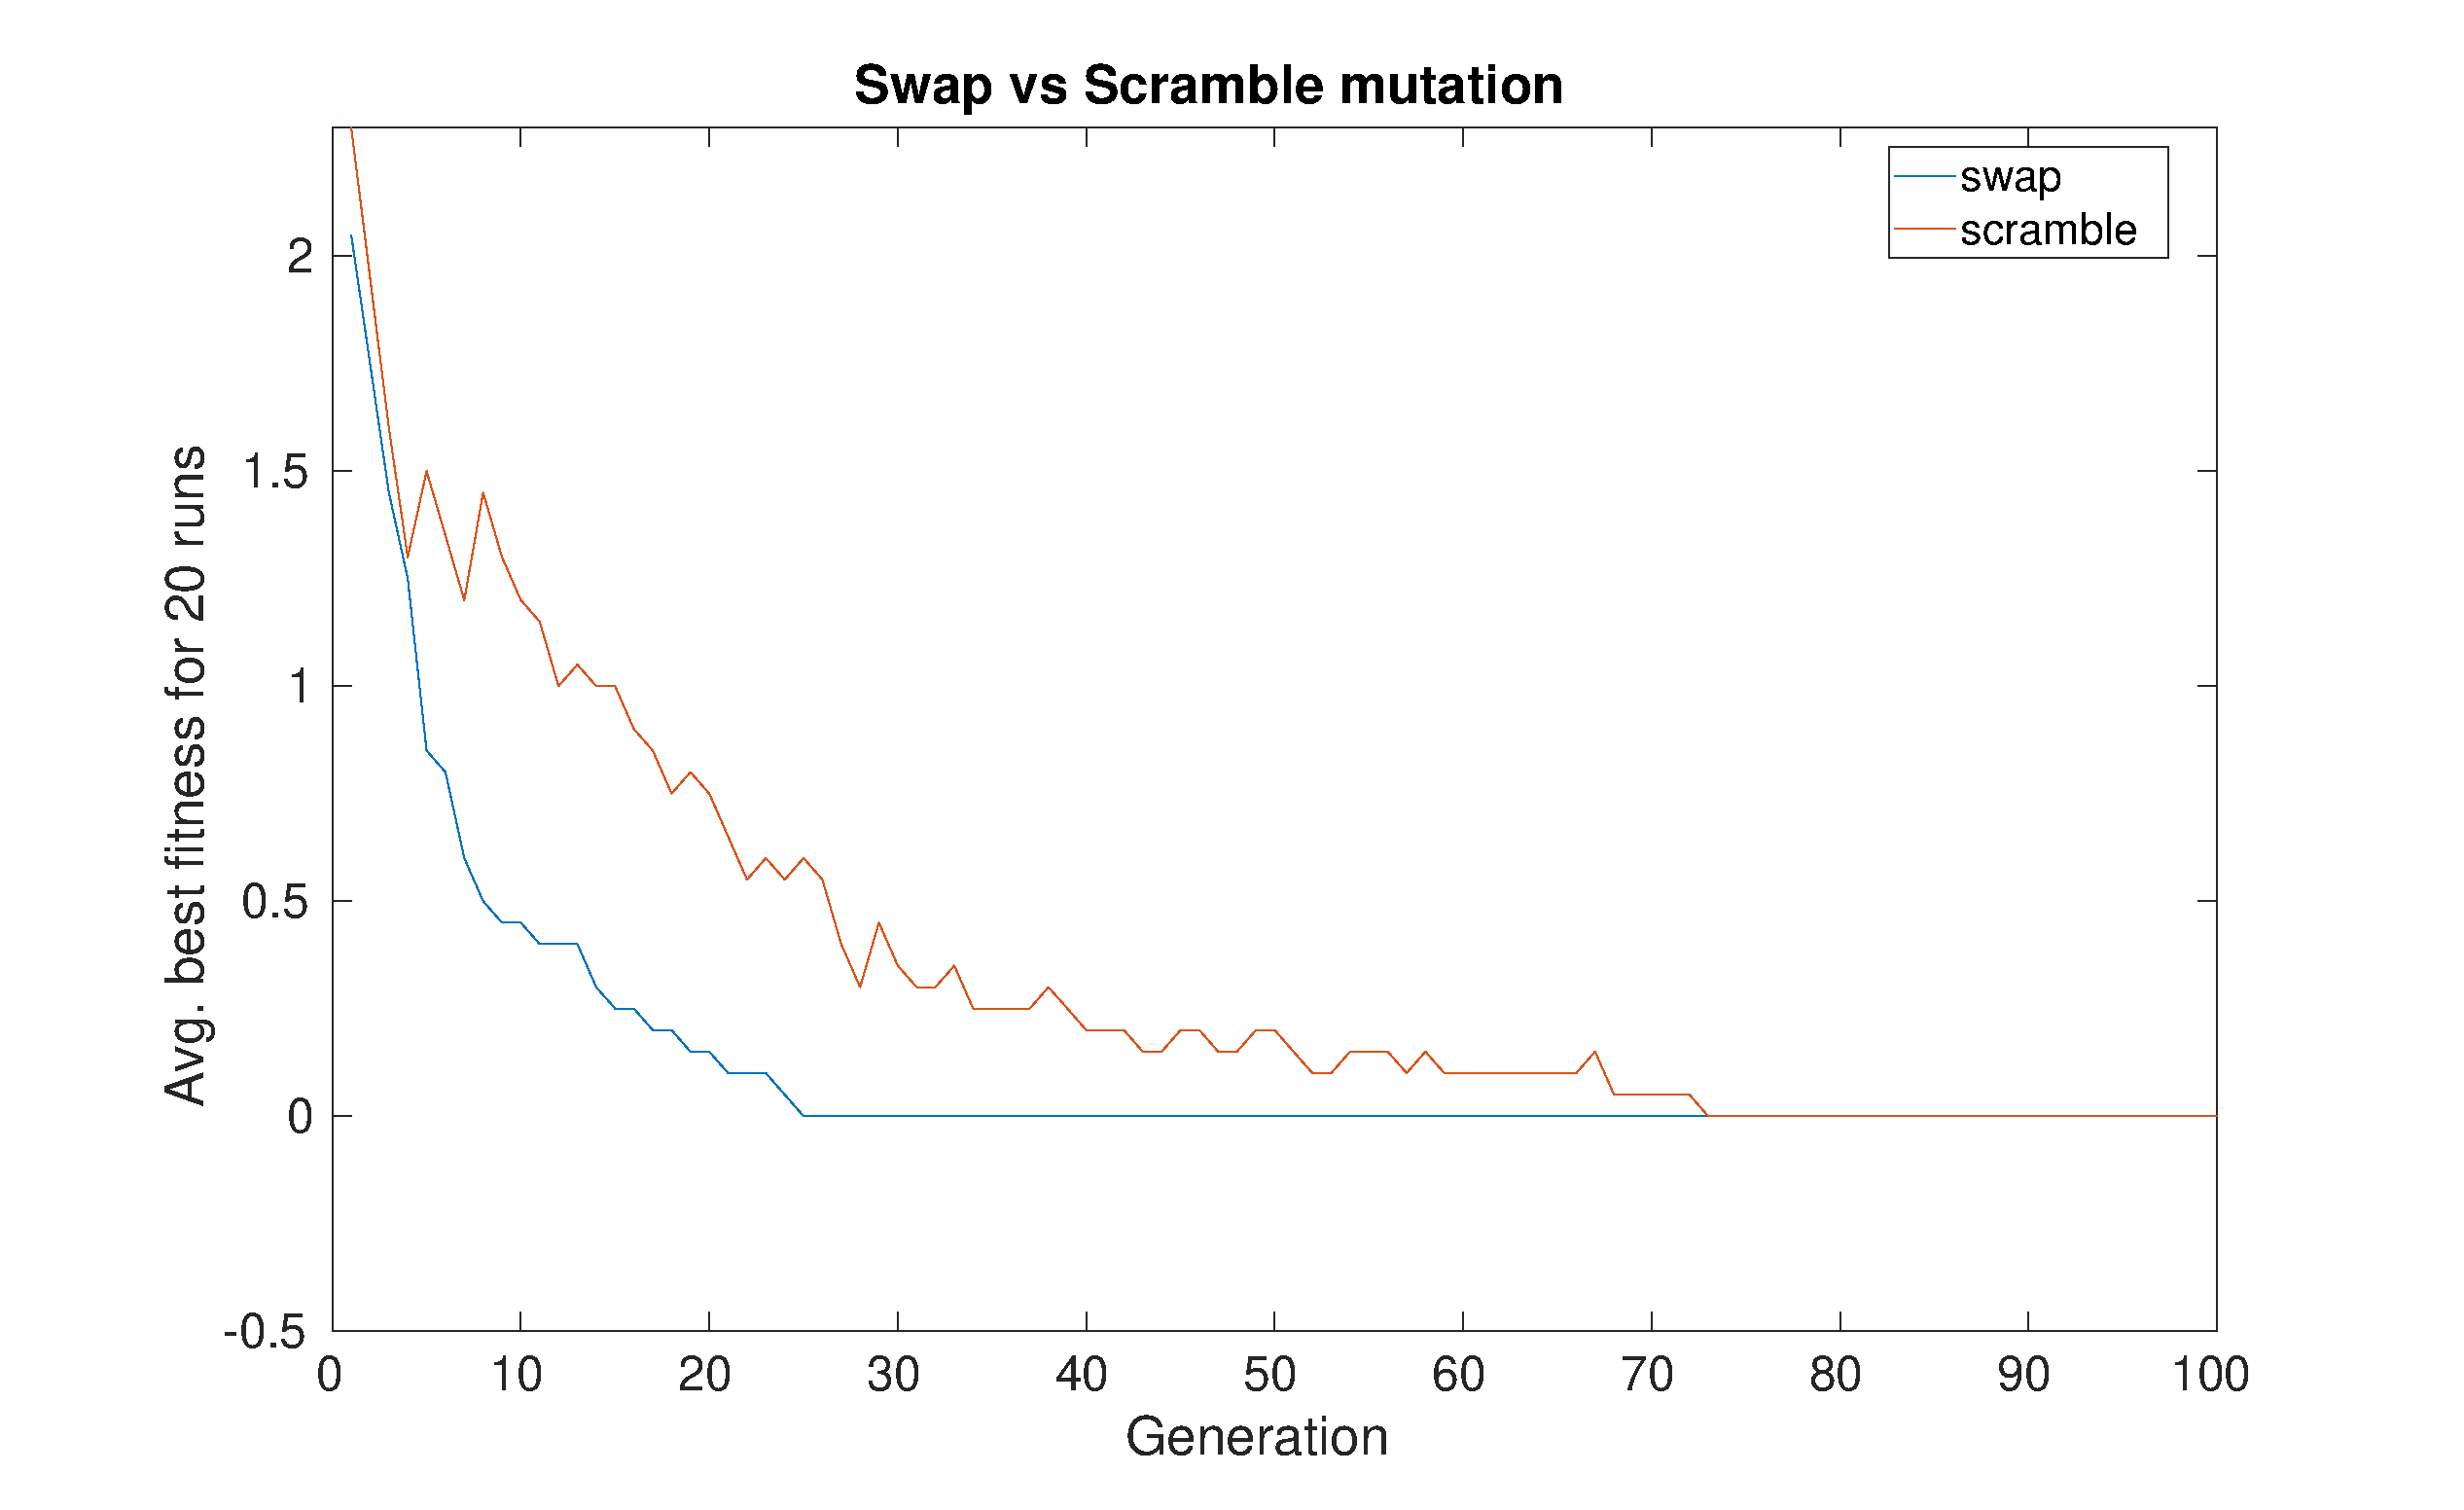
\includegraphics[width=\linewidth]{comparison_avg_fitness}
            \caption{Mutation functions' comparison by average fitness.}
            \label{fig:comp_avg_fit}
        \end{figure}

        Given both metrics' results, we can precisely affirm that swap mutation
        works better than scramble mutation in solving 16-queens problem (and
        N-queens problem in general). Swap mutation requires 4 times less
        population and 3 times less generation (therefore time) to solve the
        problem. It is pretty decent amount of resources. The reason for this
        behavior is in the nature of the problem and appliance of mutation
        functions. As for the N-queens problem, given our structure of permutations,
        it is crucially important the adjacency of the numbers and their order.
        As in scramble mutation we shuffle a big part of numbers, we corrupt
        adjacency and order. But in swap mutation, we do it gently and therefore
        we construct a new generation that is more probable to be a solution.

\end{document}
